\chapter{Stworzony system weryfikacji mówcy}\label{chap:badania}

\section{Wyczyszczenie danych}
\label{sec:data_cleaning}
% Voice Activity Detection
% wycięcie kilku o długości 1

\section{Wydobycie cech}
\label{sec:data_wrangling}

\subsection{MFCC}
% MFCC + D + DD, opis ostatecznych parametrów

\subsection{CMUDict}
% Jak zamieniłem transkrypcje w listy fonów, 39 fonów z angielskiego

\section{Wykorzystane modele}
\label{sec:data_models}

\subsectionex{Model GMM-UBM}{Mikstury gaussowskie z uniwersalny modelem tła}
\label{sec:gmm_ubm}

Pierwszym z~wykonanych w~pracy usprawnień było ujednolicenie wyświetlania rodzin
typów. Problem polegał na tym, iż w~zależności od miejsca i~rodzaju błędu,
wyświetlane były one w~różny sposób. Co gorsza, różniły się one nie tylko
formatem, ale też tym, które informacje zawierają. Widać to na poniższych
wycinkach z~komunikatów generowanych przez kompilator. We fragmencie
\ref{lst:consistent_conflicting_before}, z~błędem w~otwartej rodzinie typów,
widoczna jest lewa strona równań i~wskazania, w~którym miejscu w~pliku się one
znajdują.

\subsectionex{Model HMM-GMM}{Ukryte modele Markowa z emisjami w postaci mikstur gaussowskich}
\label{sec:gmm_ubm}

\subsectionex{Model DNN-GMM}{Głęboka sieć neuronowa do dopasowania ramek z miksturami gaussowskimi}
\label{sec:dnn_gmm}

%https://arxiv.org/pdf/1412.5567.pdf
%3 Nonrecursive -> 1 LSTM -> 1 Nonrecursive
%
%Trained on
%
%Dataset	Type	Hours	Speakers
%WSJ	read	80	280
%Switchboard	conversational	300	4000
%Fisher	conversational	2000	23000
%Baidu	read	5000	9600
%(the model available at github I think didn't include Baidu 5000 hours)

\section{Wyniki testów}
\label{sec:test_results}

Wyświetlania ostrzeżeń dokonano przez zmiany w~renamerze. Po analizie kodu udało
się stwierdzić, że funkcja \code{rnFamInstDecl} z~modułu \code{RnSource} odpowiada za wszystkie rodziny
typów w~kodzie, otwarte, zamknięte i~związane z~klasą. Ponadto jest już w~niej
używana funkcja \code{extractHsTysRdrTyVars} z~modułu \code{RnTypes}, która
przechodzi po wzorcach po lewej stronie równania,
kolekcjonując nazwy zmiennych, by utworzyć z~nich zmienne typów. Zbiór zmiennych
używanych to z~kolei to samo, co zbiór zmiennych wolnych po prawej stronie
równania, zwracany przez funkcję \code{rnPayload}. Większość informacji
potrzebnych do realizacji założeń zgłoszenia było zatem dostępnych od początku,
należało pozyskać informacje o~duplikatach.

Testami sprawdzającymi działanie usprawnienia są \code{UnusedTyVarWarnings}
i~\code{UnusedTyVarWarningsNamedWCs}. Oba działają przez próbę kompilacji pewnego
programu i~sprawdzenie, czy na wyjściu kompilatora pojawiają się oczekiwane
ostrzeżenia. Program ten zawiera jedenaście przykładów rodzin typów otwartych,
zamkniętych lub rodzin typów danych. Wśród ich równań są przypadki zmiennych
nieużywanych, używanych ze względu na wystąpienie po prawej stronie i~używanych
ze względu na wielokrotne wystąpienie po lewej stronie, z~nazwą poprzedzoną
podkreślnikiem oraz symboli wieloznacznych. Testy te różnią się od siebie tym,
iż w~przypadku \code{UnusedTyVarWarningsNamedWCs} kompilacja zachodzi
z~dodatkowo uaktywnionym rozszerzeniem \code{NamedWildCards}. Ma to związek ze zgłoszeniem
opisanym w~sekcji.


\begin{table}[H]
    \caption{Macierz $D$ dla $DTW$ na dwóch przykładowych sekwencjach $N$ i $M$. Przykład gdy elementy jednej sekwencja są wielokrotnie dopasowana do pierwszego elementu z drugiej sekwencji, dopóki jest to możliwe.}
    \centering
    \label{tab:dtw_example0}
    \small
    \tabulinesep =_3pt^3pt
    \begin{tabu}{r*{7}{r}}
        \multirow{2}{*}{} & & \multicolumn{5}{c}{N}
        \\
        & & - & 1 & 20 & 20 & 20 & 20
        \\ \midrule
        \multirow{5}{*}{M} & - & 0 & $\infty$ & $\infty$ & $\infty$ & $\infty$ & $\infty$
        \\
        & 1 & $\infty$ & 0 & 19 & 38 & 57 & 76
        \\
        & 1 & $\infty$ & 0 & 19 & 38 & 57 & 76
        \\
        & 1 & $\infty$ & 0 & 19 & 38 & 57 & 76
        \\
        & 10 & $\infty$ & 9 & 10 & 20 & 30 & \textbf{40}
        \\
    \end{tabu}
\end{table}

%\begin{figure}[H]
%    \centering
%    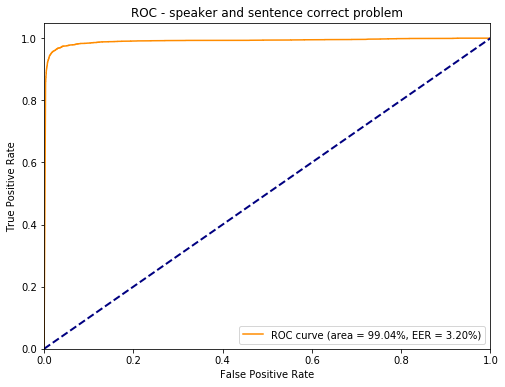
\includegraphics[width=0.8\textwidth]{images/2_2_b_roc_example}
%    \caption{Przykładowy wykres krzywej \shortcut{ROC} wygenerowany na podstawie wyników modelu \shortcut{GMM-UBM} opisanego w pracy.}
%    \label{fig:2_2_b_roc_example}
%\end{figure}

